\section{Introduction}

Automated building-maintenance systems convert photographs into tracked defect
records: a re-photographed defect must eventually be \emph{re-identified} --- matched to its
record, or given a new one. This paper first studies within-visit re-identification
under viewpoint change. Wall cracks are a common and difficult case, because
the same crack is re-photographed from different distances, angles and lighting,
and (Sec.~\ref{sec:dataset}) grows.

Crack analysis is a mature \emph{detection} and \emph{segmentation} task, and its
datasets --- CrackSeg9k~\cite{kulkarni2022crackseg9k},
OmniCrack30k~\cite{benz2024omnicrack30k} --- carry no cross-observation identity
labels, because the task they serve needs none. We know of no benchmark for crack
\emph{re-identification}; the natural approach, crop-and-match as in person and
vehicle re-ID~\cite{zhou2019osnet,qian2024reidtrends}, assumes a crack has
stable, locally distinctive appearance, and whether it does has never been
measured. We introduce \textsc{CrackID} --- 140 photographs, 17 walls, 212 crack
identities --- to make that re-identification measurement (Fig.~\ref{fig:ceiling}). Capture is one
continuous walk-around per wall, so what is measured is \emph{within-visit}
viewpoint and scale correspondence --- an upper bound on multi-visit
performance; we add a synthetic revisit protocol as a venue-controlled
secondary check (Sec.~\ref{sec:hybridbench}). That check uses a distinct
\emph{Hybrid} pipeline: it extends the Table~I \ours{} registration baseline
with a skeleton-comparison fallback and per-pair blending, so its reversal is
not a direct contradiction of Table~I.

\smallskip
\noindent\textbf{Appearance buys almost nothing on the decision.} On ranking the
nine matchers separate as expected (Rank-1 $0.352$--$0.654$ against $0.336$
chance); on pairwise $F_1$ --- the \emph{same-crack-or-not} decision a record
makes at a threshold --- all nine land between $0.000$ and $0.054$ above the
$0.305$ floor, two (ORB, DeiT) at exactly zero,
and at a validation-calibrated threshold eight of the nine span only $-0.012$ to $+0.012$
around chance while LoFTR holds a real margin of $0.046$.

\smallskip
\noindent\textbf{Two controls say where the difficulty is not.} Giving an
embedder the surrounding wall raises OSNet's open-set rate $0.168 \to 0.404$;
\emph{erasing the crack} from that view costs almost none of it ($0.393$) ---
such a method retrieves on the wall, and the cue that works, even implicitly, is
\emph{location}.

\smallskip
\noindent\textbf{A geometric baseline makes location explicit.} Registering on
non-crack texture, projecting crack masks into a common frame, and Chamfer-matching
under global assignment reaches $\mathrm{DIR}@\mathrm{FAR}{=}0.1$ of $0.768$
against $0.429$ (best crop) and $0.404$ (best context), answering $48\%$ of
pairs; a \textsc{Coverage-only} control scores $0.000$ on the same metric, so the
open-set gap is matching, not alignment coverage. This is a conditional result,
not a deployment-ready system: two test walls have zero registration success,
and the annotation and baseline both use homography-based alignment.
The resulting geometric advantage is therefore a hypothesis about this benchmark,
not an independently established identity effect.

\smallskip
\noindent\textbf{The revisit check reverses the ranking story.} The real data are
one continuous walk-around per wall, minutes apart, not separate visits. Under
the synthetic warp-plus-appearance protocol, OSNet$+$context beats the hybrid at
R@1 ($0.826/0.671$ versus $0.275/0.274$) and open-set rate
($0.739/0.663$ versus $0.343/0.342$) for growth/appearance change; the hybrid's
small assignment-$F_1$ advantage is not evidence that geometry solves real
multi-visit re-identification.

\smallskip
\noindent\textbf{Contributions:} (i)~\textsc{CrackID} with an explicit
annotation-quality report --- $45\%$ of identities were formed by an automatic
merge, reported rather than assumed (Sec.~\ref{sec:annotation}); (ii)~a
nine-method benchmark against stated chance levels, with crop$+$context and
crack-erased controls (Sec.~\ref{sec:ceiling}); (iii)~a synthetic revisit protocol isolating appearance change from damage
evolution --- the only multi-visit evidence this paper has
(Sec.~\ref{sec:hybridbench});
(iv)~a geometric reference
baseline and a protocol for this task's failure modes --- coverage-aware
metrics, unanswerable queries, an admission gate, wall-resampled confidence
(Sec.~\ref{sec:method}, \ref{sec:protocol},~\ref{sec:results}).

\begin{figure}[t]
\centering
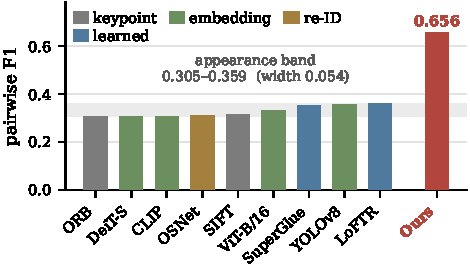
\includegraphics[width=\columnwidth]{figs/ceiling.pdf}
\caption{\textbf{The appearance ceiling.} Pairwise $F_1$ for nine crop-scope
matchers spanning four method families on \textsc{CrackID} test. Every method
falls inside the band $0.305$--$0.359$ --- width $0.054$ --- pressed against the
$0.305$ chance floor ($2p/(1+p)$ for this pool), irrespective of family, era, or
compute budget. The geometric reference baseline (red) leaves the band. Ranking
metrics separate the same methods over a $0.30$ range; the decision metric does
not.}
\label{fig:ceiling}
\end{figure}